\documentclass[12pt]{article}
\usepackage{graphicx}
\usepackage{tikz}
\title{Intermediate report iRODS}
\author{David Wouters}
\date{\today}
\begin{document}
\maketitle

\section{General comments}
\subsection{Error messages}
Overall, I'd like to say that to a regular user the error message are bulky and non-descriptive. 
I'm having a really hard time pinpointing what exactly is wrong. 
More importantly, when I start a new session, I'd say about 1 out of 5 times I get an error that the server is down, which is not really acceptable for a robust database

\begin{figure}[h!]
        \centering
        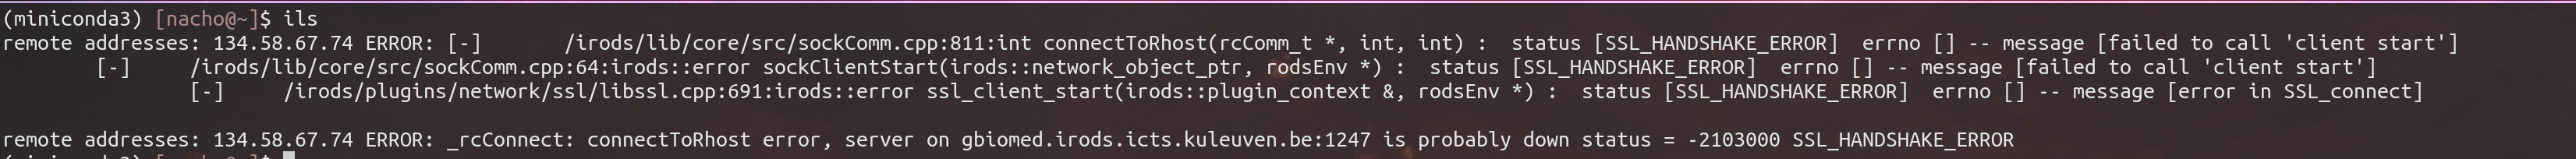
\includegraphics[width=\linewidth]{imgs/down_error.png}
\end{figure}

\section{Feature requests}
\subsection{Python iRODS Client (PRC)}%
\begin{itemize}
        \item get and put should be able to support recursive directories collecitons, havind to create that yourself is sort of tedious.
        \item I was told that glob patterns would work in the Python client. I haven't been able to make that work though.
\end{itemize}}

\subsection{Bash client}%
\begin{itemize}
        \item Tab-completion on bash command
        \item An easier way to calculate disk usage
        \item Glob patterns really need to be supported
\end{itemize}
\section{Iput report}
\begin{itemize}
        \item Large files go about as expected, however small files seem to decrease upload speed a ton.
\end{itemize}

        
\end{document}
